
\section{Spatial Closure based on the HO Solution}
\label{sec:spat_clos}

This sections describes an alternative spatial closure to the LO equations based on 
a parametric relation from the HO solution. In addition to estimating the angular
consistency terms, the HO intensity estimates a relation between volume and face-averaged
intensities to eliminate the remaining unknowns from the equations.  In the remainder of
this section, we will motivate the HO spatial closure by manipulating a half-range balance
equations to form a single unknown for each cell and half range.  We will then discuss
the forms of HO spatial closures investigated, based on modifications to standard spatial closures.

\subsection{Motivation}

A half-range balance equation for $\mu>0$ is formed by adding the
exact $L$ and
$R$ radiation moment equations given by
Eq.~\eqref{eq:exact_lmomp}~and~\eqref{eq:exact_rmomp}, i.e.,
\begin{equation}\label{eq:hr_bal}
    \mu^+_{i+1/2}\phi_{i+1/2}^+ - \mu^+_{i-1/2}\phi_{i-1/2}^+ +
    {\sigma_{a,i}h_i} \phi_i^+ = \frac{h_i}{2} q_i,
\end{equation}
where $q_i$ represents the cell-averaged emission source.  In the HOLO algorithm, after
estimating the consistency terms $\mu_{i\pm1/2}^+$ upwinding the inflow term
$\phi_{i-1/2}^+$, an additional equation is needed to eliminate the outflow $\phi_{i+1/2}^+$ to produce an
equation for a single unknown $\phi_{i}^+$.  Standard spatial discretizations techniques
use a fixed approximation for all cells to eliminate the outflow in terms of other
unknowns.  Alternatively, the HO solution can be used to estimate a parametric relation
between the other unknowns and the outflow, i.e.,
\begin{equation}\label{eq:ho_clos}
    \phi_{i+1/2}^+ = f(\gamma^{+,HO}_i, \phi_i^+, \phi_{x,i}^+, \phi_{i-1/2}^+),
\end{equation}
where $\gamma^{HO,+}_i$ is a local constant to be estimated with the HO solution and $f$ is some
function of some number of the input
variables.  The ECMC solution can provide all of the unknowns in the above equation, so
the value of $\gamma^{HO}_i$ can be determined directly. 

If the problem were linear, or the nonlinear problem was fully converged,
then application of this closure can ensure that the HO and LO equations produce the same
moments, preserving the HO accuracy.  To produce the
same moments, the HO solution must also satisfy the local balance equation, e.g.,
Eq.~\eqref{eq:hr_bal}.  Then the LO equations and HO equations must have the same moments
to satisfy both Eq.~\eqref{eq:ho_clos} and Eq.~\eqref{eq:hr_bal}, upon nonlinear
convergence of the outer HOLO iterations. If any higher moments are introduced through the spatial closure,
then the HO solution must also satisfy the corresponding balance equations that the LO
equations do.  For example, both the LO and HO equation must satisfy the
first moment equation in space if the closure is a function of the first moment.  

As TRT problems are non-linear (i.e., scattering or thermal emission are included in
$q$), the moments will only be preserved upon non-linear convergence of the source.  The
nonlinearity introduces the possibility for stability
issues, particularly with MC noise.  However, we have already consistently formed angular consistency terms, so the
the spatial closure should be more stable than introducing other terms, such as
in NDA methods~\cite{rmc,willert}. 





\subsection{Choice of Spatial Closure}
\label{sec:spat_clos_options}

We will
explore two different closure relations based on modifications to the standard LD closure: a scaled slope, i.e.,
\begin{equation}\label{eq:cl_slope1}
    \phi_{i\pm1/2}^\pm = \phi_i^+ \pm \gamma_i^{\pm} \phi_{x,i}^+
\end{equation}
and a scaled average
\begin{equation}\label{eq:cl_avg1}
    \phi_{i\pm1/2}^\pm = \gamma_i^{\pm} \phi_i^+ \pm \phi_{x,i}^+,
\end{equation}
where a value of $\gamma_i = 1$ produces the standard linear discontinuous expressions for
the extrapolated outflows.  Our LO system is formulated in terms of $L$ and $R$ moments, rather than the average and
slope.  Thus, Eq.~\eqref{eq:cl_slope1} and~\eqref{eq:cl_avg1} are expressed in terms of the $L$ and $R$
unknowns, using the relations given in App.~\ref{app:lo_mom_relations}.  In terms of these
moments, the scaled-slope closure is
\begin{align}\label{eq:cl_slope}
    \phi_{i+1/2}^+  &= \left(\frac{\ds 1 - 3 \gamma_i^+}{\ds 2 }  \right)
    \mom{\phi}_{L,i}^+ + \left(\frac{\ds 1 + 3 \gamma_i^+}{\ds 2 }  \right)
    \mom{\phi}_{R,i}^+ \\
    \phi_{i-1/2}^-  &= \left(\frac{\ds 1 + 3 \gamma_i^-}{\ds 2 }  \right)
    \mom{\phi}_{L,i}^- + \left(\frac{\ds 1 - 3 \gamma_i^-}{\ds 2 }  \right)
    \mom{\phi}_{R,i}^- 
\end{align}
and the scaled-average relation is
\begin{align}\label{eq:cl_avg}
    \phi_{i+1/2}^+  &= \left(\frac{\ds  \gamma_i^+ - 3}{\ds 2 }  \right)
    \mom{\phi}_{L,i}^+ + \left(\frac{\ds \gamma_i^+ + 3}{\ds 2 }  \right)
    \mom{\phi}_{R,i}^+ \\
    \phi_{i-1/2}^-  &= \left(\frac{\ds \gamma_i^- + 3}{\ds 2 }  \right)
    \mom{\phi}_{L,i}^- + \left(\frac{\ds \gamma_i^- - 3}{\ds 2 }  \right)
    \mom{\phi}_{R,i}^- .
\end{align}

The HO solution is used to estimate $\gamma_i$. The MC solution must be modified
to tally the MC estimated intensity on faces. For example, for $\mu>0$, the LO equations for
moments at $k+1$ use closure parameters evaluated at $k+1/2$ as
\begin{equation}
    \gamma_i^{+,HO,k+1/2} = \frac{\phi_{i+1/2}^{+,HO,k+1/2} -
    \phi_{i}^{+,HO,k+1/2}}{\phi_{x,i}^{+,HO,k+1/2}},
\end{equation}
for the scaled-slope closure.  For this closure, as the slope goes to zero this expression
becomes undefined.  In cells where the slope is $O(10^{-13} \psi_i)$, we use $\gamma_i=1$.
For the problems tested, no issues have occurred with this closure, even $\gamma$
can become very large for common, small values of $|\psi^x/\psi_i|$.  This is because in
such regions the solution is changing minimally anyways. 
The main benefit of the scaled-slope closure is it allows for values of $\gamma$ that are
equivalent to other closures, as discussed in App.~\ref{app:lo_mom_relations}:
$\gamma_i=0$ produces a step closure~\cite{larsen_edl}, which has a zero slope over the cell, and $\gamma_i=1/3$
produces a lumping-equivalent closure. 

\subsection{The Doubly-Discontinuous Trial Space}

Because of the temperature unknowns and the HO scattering source representation, a
representation on the interior of the cell for the temperature and intensity is needed.
Thus, we introduce a linear doubly discontinuous (LDD) trial space
for the half-range intensities, which is depicted in Fig.~\ref{fig:ldd_space}.  The linear
relation on the interior of the cell preserves the $L$ and $R$ moments of the solution,
and the outflow from the cell is some parametric (i.e., non linear) extrapolation of
those moments. 
The temperature is still represented with a linear interpolant of $T^4$ and $T$.  This
trial space has an extra unknown in the radiation equations for each cell and direction, which is eliminated
from the system with the HO spatial closure.  The ECMC algorithm is modified to also
include a LDD trial space which allows for estimate of the solution at faces, as discussed
later in Sec~\ref{sec:ldd_mc}. 

To solve the LO equations, Eq.~\eqref{eq:cl_slope} or~\eqref{eq:cl_avg} is substituted
locally for
the appropriate outflow face term in each LO moment equation. There is a spatial closure parameter for each
half-range, for each cell.
 The $\gamma_i^\pm$ are
estimated from the previous HO solution. For the initial LO solve within each
time step, the outflow is assumed continuous, using the standard upwinding and LD closure.  
As an example, the positive half-range and $L$ moment equation (i.e.,
Eq.~\eqref{eq:exact_lmomp}), for the scaled-slope closure, becomes
\begin{multline}
    -2{\mu}_{i-1/2}^{n+1,+} \left[\left(\frac{\ds 1 - 3 \gamma_{i-1}^{HO,+}}{\ds 2 }  \right)
        \mom{\phi}_{L,i-1}^+ + \left(\frac{\ds 1 + 3 \gamma_{i-1}^{HO,+}}{\ds 2 }  \right)
    \mom{\phi}_{R,i-1}^+
    \right] \\ + \cur {\mu}_{L,i}^{n+1,+}
  \mom{\phi}_{L,i}^{n+1,+}
  +  \cur\mu_{R,i}^{n+1,+}
  \mom{\phi}_{R,i}^{n+1,+}\\ +  \left(\sigma_{t,i}^{n+1}+\frac{1}{c \Delta t} \right) h_i 
  \mom{\phi}_{L,i}^{n+1,+} -  \frac{\sigma_{s,i} h_i}{2} \left( \mom{\phi}_{L,i}^{n+1,+} +
  \mom\phi_{L,i}^{n+1,-}\right)\\  = \frac{h_i}{2} \mom{\sigma_a^{n+1} a c T^{n+1,4}}_{L,i} +
  \frac{h_i}{c\Delta t}\mom{\phi}_{L,i}^{n,+},
    \label{eqn:clsd_posl}
\end{multline}
and the $R$ moment equation becomes
\begin{multline}
    2{\mu}_{i+1/2}^{n+1,+} \left[
    \left(\frac{\ds 1 - 3 \gamma_{i}^{HO,+}}{\ds 2 }  \right)
        \mom{\phi}_{L,i}^+ + \left(\frac{\ds 1 + 3 \gamma_{i}^{HO,+}}{\ds 2 }  \right)
    \mom{\phi}_{R,i}^+
    \right]  \\ 
    - \cur {\mu}_{L,i}^{n+1,+}
  \mom{\phi}_{L,i}^{n+1,+}
  -  \cur\mu_{R,i}^{n+1,+}
  \mom{\phi}_{R,i}^{n+1,+} +  \left(\sigma_{t,i}^{n+1}+\frac{1}{c \Delta t} \right) h_i 
  \mom{\phi}_{R,i}^{n+1,+} \\-  \frac{\sigma_{s,i} h_i}{2} \left( \mom{\phi}_{R,i}^{n+1,+} +
  \mom\phi_{R,i}^{n+1,-}\right) = \frac{h_i}{2} \mom{\sigma_a^{n+1} a c T^{n+1,4}}_{R,i} +
  \frac{h_i}{c\Delta t}\mom{\phi}_{R,i}^{n,+}.
    \label{eqn:clsd_posr}
\end{multline}
These equations contain only the original desired radiation moment and LD temperature unknowns.
During the Newton solve, once new half-range
intensities are determined, the temperatures are updated using the same material
energy equations as for the LD closure, i.e., Eq.~\eqref{eq:lo_mat_dis1} and Eq.~\eqref{eq:lo_mat_dis2}.

Because the
outflow from one cell is upwinded into the next cell, energy conservation by the LO
equations is preserved.
The closed equations have the
same numerical complexity as the LDFE LO equations, but with an increased storage on the
coarse mesh for the
$\{\gamma_i\}$.  Also, the linear representation for the interior
solutions and emission source should approach the LD closure in the equilibrium diffusion limit, as long
as the HO spatial closure is estimated with sufficient statistical accuracy.  

\subsubsection{Fixups for Negative Solutions}

In the case of strong gradients, the interior representation could be driven
negative.  In such cases, we can use the lumping-equivalent relation from
App.~\ref{app:lo_mom_relations} to define the linear representation.  For
example, the lumped emission source is
\begin{equation}
    T = \mom{T}_{L,i}^4 b_{L,i}(x) + \mom{T}_{R,i}^4 b_{R,i}(x) , \quad x\in(\xl,\xr)
\end{equation}
There are analogous relations for $T(x)$ and $\phi^\pm(x)$ over each cell.
These expressions are positive as long as the moments are positive, which is true for
physical solutions.  If the lagged, MC spatial closure produces an outflow from a cell that is
negative, then these moments could become negative.  In such cases, we force that cell to
use a standard lumped relation for the moment equations, with no discontinuity at the
outflow, and restart that Newton solve.  It is important to note that the spatial closure will still have the same
relation between the moments and the outflow; the lumping relation only affects the
linear representation that the moments correspond to.  For example in
Eq.~\eqref{eq:lo_mat_dis1}, the lumped representation changes $2/3
T_{L,i} + 1/3 T_{R,i}$ to $T_{L,i}$, but no modification are made to the
absorption term $\sigma_{a,i}\mom{\phi}_{L,i}$.

%During the Newton solve, once new half-range
%intensities are determined, the temperatures are updated using the material energy
%moment equations, i.e., Eq.~\eqref{eq:lo_mat_dis1} and Eq.~\eqref{eq:lo_mat_dis2}. For the
%uulumped case, the radiation moments are the same.  he slope moment,
%e.g., $\psi_{x,i}^\pm$, does not strictly correspond to the slope in the typical since.
%We have modified it in the lumped relation.  This is the same as the lumped closure relation using
%$\gamma_i=1/3$, where we are preserving the average moment exactly, but only second order
%accurate in the slope.

\begin{figure}[H]
    \centering
    {\resizebox{0.5\textwidth}{!}{
        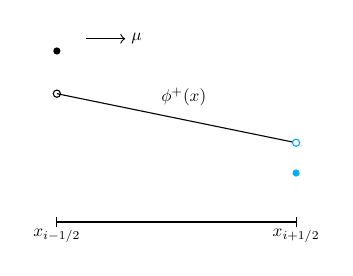
\begin{tikzpicture}[scale=0.62, every node/.style={transform shape}]
            \draw (1.0,4.0) node[fill,circle,inner sep=0pt,minimum
            size=4.2pt] {};
            \draw [->] (1.6,4.25) -- (2.4,4.25) node[anchor=west] {$\mu$};
            \draw (1.0,0.4) -- (1.0,0.6) node[below, pos=0.4] {$x_{i-1/2}$};
            \draw (5.90,0.4) -- (5.90,0.6) node[below, pos=0.4] {$x_{i+1/2}$};
            \node at (3.6,3.06) {$\phi^+(x)$};
            \draw [thick] (1.0,0.5) -- (5.9,0.5) node[anchor=north west] {};
            \filldraw[color=black, fill=white] (1,3.1250) circle (2.1pt);
            \draw (1.0,3.125) -- (5.90,2.120);
            \filldraw[color=cyan, fill=white] (5.9,2.120) circle (2.1pt);
            \draw (5.9,1.5) node[cyan,fill,circle,inner sep=0pt,minimum size=4.2pt] {};
        \end{tikzpicture}
    }}
    \caption{Linear doubly-discontinous representation for mean intensity in LO equations.     \label{fig:ldd_space}}
\end{figure}


\subsection{Issues with ECMC for Spatial Closure}
\label{sec:ecmc_issues}
There are several issues with ECMC that cause the LO moments to not exactly preserve
the HO moments, even for a linear problem.  With ECMC, global and, particularly, local
energy balance are generally not preserved.  For standard MC, there
are source biasing techniques (e.g., systematic
sampling) that exactly preserve the local zeroth moment of the
source and thus satisfy the local balance equations~\cite{shultis_mc,wollaber_review}). 
However, for our HOLO method, even with standard MC we have to reconstruct the bilnear moment
of $x$ and $\mu$, so the consistency terms lead to LO equations that do not exactly
preserve the first moment of the HO solution\footnote{It was verified that with
standard MC, systematic sampling, no analog sampling, and a closure that is only a
function of the zeroth moment, the LO solution exactly reproduces the HO moments, for
a linear problem}.  One final reason is that the analog treatment of absorption for
particles below the weight cutoff (e.g., see Sec.~\ref{sec:tallies}) results in
$\sigma_a \phi^{HO}_i$ and the amount of energy removed from a cell during MC
transport to not be equal; this is due to statistical noise in the path-length
estimators for $\phi^{HO}_i$.  However, ECMC will preserve balance to the order of
the iterative error and statistical noise, so the closure parameters will reproduce
the HO moments to the accuracy of the LO solution.  

\section{Test Problems}

To investigate the utility of the face closures we compare to the LD spatial
closure for two test problems.  We are interested in the accuracy of the solution and
consistency between the HO and LO solutions, particularly for coarser meshes. 
The consistency for the $(l)$-th particular simulation is measured with the relative L$_2$ norm
of the difference between the projected HO and LO solutions, i.e.,
\begin{equation}
    \|\phi_{HO} - \phi_{LO}\|^{(l)}_{2,rel} = \frac{\ds \sqrt{\int_0^X \left(
        \phi_{HO}^{(l)}(x) - \phi_{LO}^{(l)}(x) \right)^2 \dd x}}{\ds \sqrt{
            \int_0^X \left(\phi_{LO}^{(l)}(x)\right)^2 \dd x }}
\end{equation}
where $\phi_{LO}(x)$ and $\phi_{HO}(x)$ are the LDFE representations in space of the
intensity from the HO and LO solvers, from the end of the last time step.
The error between a reference solution and a fine solution for the ${(l)}$-th simulation
is computed as
\begin{equation}
    \|e\|^{{(l)}}_{2,rel} = \frac{\|\phi_{LO}^{n+1,{(l)}}(x) -
    \phi_{LO}^{n+1,ref}\|}{\|\phi_{LO}^{n+1,ref}\|}
\end{equation}
All L$_2$ norms are computed using quadrature over the finest spatial mesh.  An
integrated measure of the error in cell-averaged mean intensities on the mesh of the
$l$-th simulation, with $N_c^{(l)}$ spatial cells, is computed as
\begin{equation}
    \|e\|^{{(l)}}_{a,rel} = \left({\frac{\ds \sum\limits_{i=1}^{N^{(l)}_c}
    \left(\phi_i^{n+1,{(l)}} - \phi_i^{n+1,ref}
\right)^2}{\ds \sum\limits_{i=1}^{N^{(l)}_c}\left(\phi_i^{n+1,ref}\right)^2}}\right)^{1/2},
\end{equation}
where $\phi_i^{n+1,ref}$ is computed by spatially averaging the fine mesh solution over
the $i$-th coarse spatial cell.

The sample mean of each of the above metrics is estimated based on 20 independent
simulations; the sample standard deviation for each \emph{mean} is also reported, e.g.,
\begin{equation}
    s\left(\|e\|_{2,rel}\right) = \left[\frac{1}{20-1}\sum_{l=1}^{20} \left(
    \|e\|_{2,rel}^{(l)} - \|e\|_{2,rel} \right)^2\right]^{1/2},
\end{equation}
where $\|e\|_{2,rel}=\sum_{l=1}^{20}\|e\|_{2,rel}^{(l)}/20$ is the mean.

\subsection{Smooth Problem}

For this problem, the radiation and material energies are initially in
equilibrium at $0.01$ keV.   An isotropic incident intensity of 50 eV is applied
at $x=0$; the incident intensity on the right boundary is $10$ eV.
The material properties are $\rho = 1$ g cm$^{-3}$, $c_v = 0.2$ jks/keV-g, and
$\sigma_a=10$ cm$^{-1}$.
The simulation end time is 0.5 sh.  The time step size increases by 10\% each time step
until the maximum step size of 0.01 sh is reached, beginning from $\Delta t = 0.001$ sh.
This problem is intended to have less steep gradients in the intensity by having constant constant cross
sections, a smaller boundary source, and diffusive problem parameters.
The problem has a smaller optical thickness than other problems tested so that the face-based solutions can be efficiently
estimated, but the small c$_v$ value makes the solution relatively diffusive.  This
problem did not require the lumped relation to produce positive solutions.
However, when projecting from a refined mesh back to the coarse mesh, it was
necessary to rotate the solution to be positive.

All simulations of this problem used 585,900 histories divided over 9 ECMC
batches;  beginning from 30,000 histories and $10$ $\mu$ cells, 30\% of cells were
adaptively refined every third batch, and the number of histories is increased to
keep the average number of histories per cell constant. 
We have have performed two outer HOLO iterations over each time step for all cases; it was
found that additional iterations did not increase consistency, because of the  magnitude
of statistical noise.  Relative convergence of HOLO iterations was below 10$^{-3}$
for two iterations for all cases.  
Fig.~\ref{fig:smooth_compare} compares cell-averaged radiation temperatures for various spatial closures at
coarse mesh sizes and a fine-mesh solution.  The HO spatial closures curve is for the
scaled-slope closure given by Eq.~\eqref{eq:cl_slope}.  There was visually
no difference in the results between the scaled-averaged, scaled-slope, or LD closure. A step closure in all cells
was inaccurate for this problem.

Table~\ref{tab:smooth} compares the different error metrics for different spatial
closures and numbers of cells.  The reference solution for all calculations was the average of 10 simulations with $N_c=500$ spatial
cells.  In all cases, the HO spatial closure produces higher accuracy in the L$_2$
norms and greater consistency between the solvers.  However, there is not an
improvement in accuracy of the cell-averaged intensities.  Neglecting noise, the LDFE representation can be third order
accurate for the $\|e\|_a$ norm and second-order accurate in the L$_2$ norm~\cite{morel_ldtrt}. 
The statistical noise induced in face tallies makes the
additional accuracy that the MC transport can use not greater than the benefit of
higher spatial integration by the MC transport.  It
is noted that, overall, there is very low statistical noise in each of these
solutions due to the ECMC method and relatively high number of histories; at lower
history counts, the small gains of the HO spatial closure will degrade and stability
becomes an issue.

\begin{figure}[H]
    \centering
    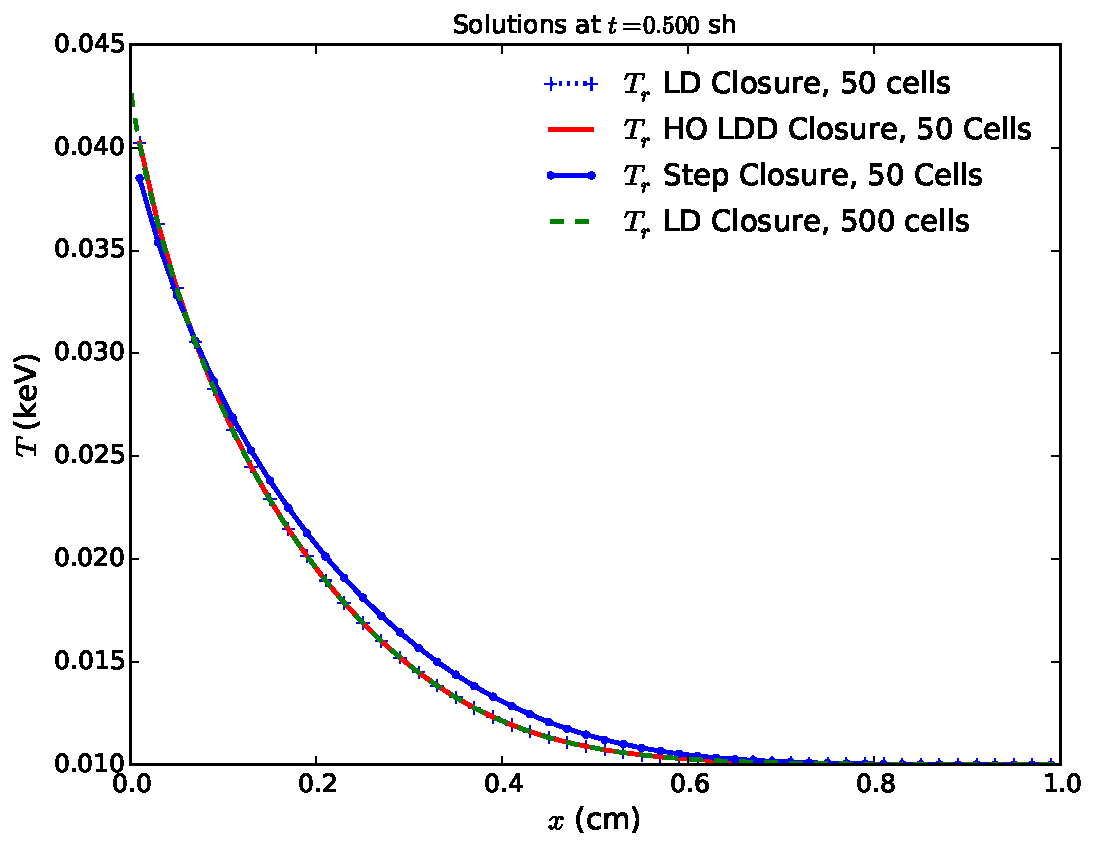
\includegraphics[width=0.99\linewidth]{smooth_compare.pdf}
    \caption{\label{fig:smooth_compare} Comparison of solutions for different spatial closures.}
\end{figure}

\begin{table}[H]
    \caption{\label{tab:smooth} Comparison of error metrics, reported as percentages, averaged over 20 simulations of smooth problem.  The absolute
standard deviation for each value is reported in parenthesis. Reference solution uses 500 cells.}
    \begin{tabular}{|l|cl|cl|cl|} \hline
        Spatial Closure & \multicolumn{2}{|c|}{$\|e\|_2$}  & \multicolumn{2}{|c|}{$\|e\|_{a}$} & \multicolumn{2}{|c|}{$\|\phi^{HO}
        -\phi^{LO}\|_{2}$} \\  \hline \hline
        \multicolumn{7}{|c|}{$N_c = 20$ cells} \\ \hline
LDFE               &   6.60\%  &   (0.17\%)  &   2.80\%     &   (5.7e-03\%)  &   2.90\%   &  (8.1e-03\%)  \\
HO: Scaled Slope   &   6.10\%  &   (2.9e-03\%)  &   3.50\%  &   (5.8e-03\%)  &   0.021\%  &  (8.6e-03\%)  \\
HO: Scaled Average &   6.10\%  &   (2.7e-03\%)  &   3.50\%  &   (5.0e-03\%)  &   0.023\%  &  (1.1e-02\%)  \\ \hline
       \multicolumn{7}{|c|}{$N_c  = 50$ cells}   \\ \hline
LDFE               &   1.60\%  &   (7.9e-04\%)  &   0.59\%  &   (3.8e-03\%)  &   0.76\%)  &  (4.8e-03\%)  \\
HO: Scaled Slope   &   1.40\%  &   (1.5e-03\%)  &   0.67\%  &   (3.2e-03\%)  &   0.012\%  &  (4.0e-03\%)  \\
HO: Scaled Average &   1.40\%  &   (1.5e-3\% ) &   0.67\%   &   (3.1e-03\%)  &   0.013\%  &  (3.9e-03\%)  \\ \hline
       \multicolumn{7}{|c|}{$N_c  = 100$ cells}   \\ \hline
LDFE               &   0.53\%  &   (2.1e-03\%)  &   0.15\%  &   (2.5e-03\%)  &   0.30\%)  &  (9.7e-03\%)  \%\\
HO: Scaled Slope   &   0.45\%  &   (1.5e-03\%)  &   0.16\%  &   (4.6e-03\%)  &   0.012\%  &  (4.8e-03\%)  \\
HO: Scaled Average &   0.45\%  &   (1.4e-03\%)  &   0.16\%  &   (4.7e-03\%)  &   0.012\%  &  (3.6e-03\%)  \\ \hline
    \end{tabular}
\end{table}



\section{Two Material Problem}

The HO spatial closures were applied to solution of the two material problem detailed in Sec.~\ref{sec:two}.
For these results, the time step size is increased from 0.001 sh to a maximum step of 0.01 sh by 5\% each
step, with the final step adjusted to end at 2 sh.

The scaled-slope closure was found to not stably converge, even for 3 batches of 10$^6$
histories.  This coudl be caused the steep gradients at the foot of the wave.  As the
solution slightly overshoots, the slope changes signs between cells. 

